\textit{Gradient Boosting Machines} (GBM) é um algoritmo de aprendizado de máquina, baseado na ideia de modelos aditivos de estatística e descida de gradiente. O GBM funciona construindo um modelo aditivo avançado \textit{stagewise} realizando gradiente descendente no espaço de função, conforme proposto por \cite{greedy}. O \textit{Gradient Boosting} é um algoritmo de aprendizado de máquina amplamente utilizado devido à sua eficiência, precisão e interpretabilidade.
\section{Additive Model}
Um modelo aditivo é uma técnica de regressão onde a ideia básica é aproximar um conjunto de dados usando uma soma de funções suaves do indivíduo características dos dados observados, em vez de uma superfície de regressão geral complexa \cite{persu:regre}.

Considere o conjunto de dados $\{(\mathbf{x}^{(1)},y^{(1)}),(\mathbf{x}^{(2)},y^{(2)}),...,(\mathbf{x}^{(i)},y^{(i)})\}$, em que $\mathbf{x}$ são os preditores e $y$ a saída, o modelo aditivo pode ser escrito da seguinte forma

\begin{equation}
    E|y^{(i)}|x^{(1)},x^{(2)},...,x^{(i)}| = \beta_0 + \sum_{j=1}^pf_j(x^{(ij)})
\end{equation}
Ou
\begin{equation}
    Y = \beta_0 + \sum_{j=1}^pf_j(\mathbf{X}^{(:,j)}) + \epsilon
\end{equation}
As funções $f_j(x^{(ij)}$ são conhecidas como funções de suavização, ou seja, ao invés de utilizar uma regra complexa de regressão, usamos a soma de funções de suavização.

\section{\textit{Gradient Descent}}
Podemos separar os métodos de solução de problemas de otimização entre determinísticos e métodos estocásticos. Abordagens determinísticas são geralmente mais simples que as estocásticas, porém, o risco de ficar preso em um mínimo local é significativamente maior. O gradiente descendente é um método estocásticos.

\begin{figure}[h]
 \caption{Exemplo de otimização pelo gradiente descendente.}
 \label{fig:ex:grad}
 \centering
 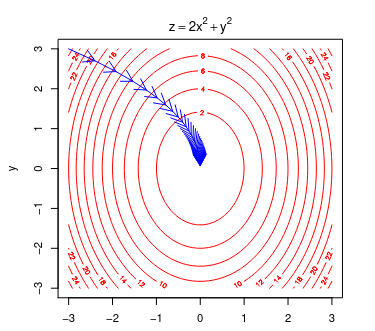
\includegraphics[scale=0.4]{images/ilustra_grad.png}
\end{figure}

A versão básica do algoritmo tem como objetivo minimizar uma função objetiva $F(\theta)$. Esse algorítimo tem uma taxa de aprendizado\simbolo{\eta,LR}{\textit{learning rate}, taxa de aprendizado}$\eta$ para controlar o quanto os coeficientes de $\theta$ podem mudar em cada interação \cite{russel,hastie,ian,over:gradia,mit:parallel,convex:opt}. 

Podemos escrever o gradiente descendente como:
\begin{equation} \label{eq:gradiente}
    \theta_t = \theta_{t-1} - \eta \cdot \nabla{\theta_{t-1}}F(\theta_{t-1};\mathbf{x}^{(i)},y^{(i)})
\end{equation}

Uma execução de descida de gradiente executará a atualização acima $t = M$ vezes e pode ser interpretada como $M$,a atualização, gerando vetores $v_m$ da forma $v_m = - \eta \cdot \nabla{\theta_{t-1}}F(\theta_{t-1};\mathbf{x}^{(i)},y^{(i)})$. Denotando $v_0 = \theta_0$, os valores iniciais dos parâmetros antes da otimização, os parâmetros finais podem ser escritos como:
\begin{equation}
    \theta^* = \sum_{m=0}^{M-1}v_m
\end{equation}



\section{\textit{Boosting}}
\textit{Boosting} é uma das ideias de aprendizado mais poderosas introduzidas nas últimas décadas. Ele foi originalmente projetado para problemas de classificação mas pode ser utilizado para problemas de regressão.  A ideia por tras do \textit{boosting} é combinar a saídas de muitos classificadores “fracos” para produzir um “comitê” poderoso, ou seja, criar um aprendiz "poderoso" a partir de uma combinação de aprendizes "fracos" \cite{brief:intro:boost,hastie}.

Um classificador fraco é aquele cuja taxa de erro é apenas ligeiramente melhor do que uma adivinhação aleatória. O objetivo do \textit{boosting} é aplicar sequencialmente o
algoritmo de classificação "fraco" para várias versões, produzindo assim uma sequência de classificadores fracos $G_m(x),m= 1, 2, 3, ..., M$.
As previsões de todos eles são combinadas por meio de uma ponderação para produzir a previsão final:
\begin{equation}
    G(x) = sign(\sum_{m=1}^M\alpha_mG_m(x))
\end{equation}

Em que $\alpha_1,\alpha_2, \alpha_M$ são calculados pelo algoritmo de boosting e cada contribuição segue um peso em $G_m(x)$. Esse algoritmo mostrado pela equação acima é conhecido como AdaBoost \cite{adaboost}. Abaixo temos um esquemático de como os classificadores são treinados na versão com peso do conjunto de dados e depois combinado com a predição final.
\begin{figure}[h]
 \caption{Esquemático do algoritmo AdaBoost \cite{hastie}.}
 \label{fig:ex:adaboost}
 \centering
 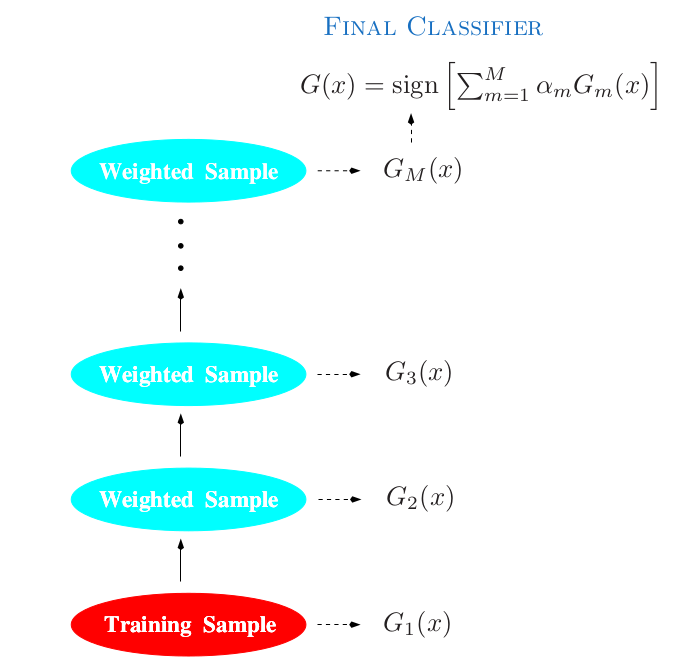
\includegraphics[scale=0.3]{images/adaboost.png}
\end{figure}

O algoritmo \ref{algoritmo:adaboost} mostra o detalhe do algoritmo de AdaBoost \cite{adaboost,hastie}.
\begin{algorithm}[H]
\caption{AdaBoost M1}\label{algoritmo:adaboost}
\begin{algorithmic}[1]
\State Iniciar as observações com pesos $w_i = 1/N, i=1,2,3,...,N$
\State \For{$m=1$ até $M$:}
\State Fit o classificador $G_m(x)$ no conjunto de treino utilizando os pesos $w_i$
\State calcule o erro $err_m = \frac{\sum_{i=1}^Nw_i\mathbf{1}(y_i\neq G_m(x_i))}{\sum_{i=1}^Nw_i}$
\State Calcule $\alpha_m = log((1-err_m)/err_m)$
\State $w_i \rightarrow w_i\cdot exp[\alpha_m \cdot \mathbf{1}(y_i\neq G_m(x_i))],i=1,2,...,N$
\EndFor
\State \Return $G(x) = sign(\sum_{m=1}^M\alpha_mG_m(x))$
\end{algorithmic}
\end{algorithm}

\section{GBMs}
\textit{Gradient Boosting Machine} utiliza o conceito de modelo aditivo e é uma combinação do gradiente descente com o \textit{boosting} \cite{greedy}. O algoritmo GBM funciona otimizando qualquer função de perda diferenciável, usando Gradiente descendente. No entanto, a otimização não é feita em termos de otimização numérica (ou seja, atualizando um vetor de parâmetros $\theta$), mas por funções de "bossting" na direção do gradiente da função de perda. Como os GBMs lidam com dados finitos, eles otimizam as funções em termos do conjunto de dados supervisionado, nosso conjunto $(\mathbf{x}^{(i)} , y^{(i)})$, o modelo final de GBM será:

\begin{equation}
    F_M(x) = F_0(x) + \sum_{m=1}^MF_m(x)
\end{equation}

As funções $F_m(x)$ são funções construídas de forma \textit{stagewise}, assim como o $\theta_t$ em gradiente descendente. As funções base são aprendizes, e podem ser parametrizadas como $\beta_m h(\mathbf{x};a_m)$, onde $\beta_m$
é um peso, e $\alpha_m$ os parâmetros do aprendiz $h$. Na maioria das implementações, as funções básicas são aprendizes baseados em árvore, mas podem ser qualquer aprendiz em que seja seja possível atribuir pesos. Também, dada uma função de perda $L(y_i , F_m(x_i))$, gostaríamos de encontrar todos os valores ótimos de $\beta_m$ e $\alpha_m$ que minimizam a função perda, ou seja:
\begin{equation*}
    \{\beta_m,\alpha_m\}_1^M = {\arg\min}_{\{\beta'_m,\alpha'_m\}_1^M}\sum_{i=1}^n L\Biggl(y^{(i)},\sum_{m=1}^M\beta'_mh(\mathbf{x}^{(i)};\alpha'_m)\Biggl)
\end{equation*}
No entanto, na maioria das situações, a otimização acima é inviável, portanto, a abordagem \textit{"greedy-stagewise”} é otimizar cada par $\beta_m$ e $\alpha_m$ em um modelo \textit{stagewise}, ou seja, para cada $m = 1, 2, ..., M$.
\begin{equation}\label{eq:interacoes}
    (\beta_m,\alpha_m) = {\arg\min}_{\beta,\alpha}\sum_{i=1}^n L\Biggl(y^{(i)},F_{m-1}\mathbf{x}^{(i)} + \beta h(\mathbf{x}^{(i)};\alpha)\Biggl)
\end{equation}
Utilizando a notação vetorizada 
\begin{equation}
    F_m(\mathbf{X}) = F_{m-1}(\mathbf{X}) + \eta \Delta_m(X)
\end{equation}
$\beta_m h(\mathbf{x}^{(i)};\alpha_m)$ pode ser interpretado como o melhor passo "greedy" em direção à estimativa, $F^*(x)$, esta pode ser vista como uma atualização do método do gradiente descendente. O análogo de $\nabla{\theta_{t-1}}$ no gradiente descente numérico é o gradiente da função de perda $L$ com relação à última estimativa $F_{m−1}(x)$ \cite{greedy}.

\begin{equation}
    -g_m(\mathbf{x}^{(i)}) = -\Bigg[\frac{\partial L(y^{(i)},c^{(i)})}{\partialF(\mathbf{x}^{(i)})}\Bigg]
\end{equation}
Em que $F(x)=F_{m-1}(x)$.

Na literatura, esse gradiente da função de perda $L$ em relação à última previsão $\hat{y}_{m−1}$. Essa última previsão às vezes é chamada de pseudo-residual e definida como $\mathbf{r}_{m-1}$. 
\begin{equation}
    \mathbf{r}_{m_1} = \nabla F_{m-1}(\mathbf{X})L(y,F_{m-1}(\mathbf{X})) = \nabla \hat{y}_{m-1}L(y,\hat{y}_{\mathbf{m-1}})
\end{equation}

O algoritmo GBM ajusta um aprendiz $h(x;\alpha_m)$ com peso $\beta$ usando os pseudo-resíduos, não o $\mathbf{X}$ original. A versão final do algoritmo é definida como:

\cite{hastie,greedy}.
\begin{algorithm}[H]
\caption{Gradient Boost($\mathbf{X},y,M,\eta$)}\label{algoritmo:gradboost}
\begin{algorithmic}[1]
\State $F_0(\mathbf{X} = \arg\min_v\sum_{i=1}^n L(y^{(i)},v)$
\State \For{$m=1$ até $M$:}
\State $\mathbf{r}_{m_1} = \nabla \hat{y}_{m-1}L(y,\hat{y}_{\mathbf{m-1}})$ \Comment{Treinar o aprendiz base para minimizar o erro quadrático}
\State $\alpha = {\arg\min}_{\alpha,\beta}\sum_{i=1}^n(\mathbf{r}_{m-1}^{(i)}-\beta h(\mathbf{x}^{(i)};\alpha))^2$
\State $\beta = {\arg\min}_{\beta}\sum_{i=1}^nL(y^{(i)},F_{m-1}(\mathbf{x}^{(i))}+\beta h(\mathbf{x}^{(i))};\alpha_m)$
\State $\Delta_m(X) = \beta_mh(\mathbf{X};\alpha_m)$
\State $F_m(\mathbf{X}) = F_{m-1}(\mathbf{X}) + \eta \Delta_m(X)$
\EndFor
\State \Return $F_m$
\end{algorithmic}
\end{algorithm}

\section{XGBoost, CatBoost e LightGBM}
Os três algoritmos no escopo do trabalho: XGBoost (\textit{Xtreme Gradient Boosting}), CatBoost (\textit{Category Boosting}) e LightGBM (\textit{Light Gradient Boosting Machine}) são todos variantes de algoritmos de \textit{Gradient Boosting}. Todos podem ser utilizados como Regressor (prevendo variáveis contínuas) ou um Classificador (prevendo variáveis categóricas).

XGBoost é uma solução altamente escalável, flexível e versátil, foi projetado para explorar recursos corretamente e superar as limitações do aumento de gradiente anterior. A principal diferença entre XGBoost e outros algoritmos de gradiente é que ele usa uma nova técnica de regularização para controlar o overfitting. Portanto,
é mais rápido e mais robusto durante o ajuste do modelo. A técnica de regularização é feita adicionando um novo termo a função de perda, como:

\begin{equation}
    L(\phi) = \sum_{i=1}^nL(\hat{y}_i,y_i) + \sum_{m=1}^M\Omega(f_k)
\end{equation}

Em que :
\begin{equation}
    \Omega(f) = \gamma T + \frac{1}{2}\lambda||w||^2
\end{equation}


XGBoost usa um novo ganho
\begin{equation} \label{eq:gain}
    Gain = \frac{1}{2}\Bigg[ \frac{(\sum_{i\in I_L}g_i)^2}{\sum_{i\in I_L}h_i + \lambda} + \frac{(\sum_{i\in R_L}g_i)^2}{\sum_{i\in R_L}h_i + \lambda} - \frac{(\sum_{i\in I}g_i)^2}{\sum_{i\in I}h_i + \lambda} \Bigg] - \gamma
\end{equation}

Em que
\begin{equation}
    g_i = \partial_{\hat{y}_i}L(\hat{y}_i,y_i) \\ 
    h_i = \partial^2_{\hat{y}_i}L(\hat{y}_i,y_i)
\end{equation}
Assuma que $I_L$ e $I_R$ são os conjuntos de instâncias da esquerda e nós direitos após a divisão e $I = I_L\cup I_R$ \cite{article:xgboost,doc:xgboost}.

\begin{figure}[H]
 \caption{Exemplo do cálculo da estrutura do cálculo do score para uma árvore \cite{article:xgboost}.}
 \label{fig:ex:xgboost}
 \centering
 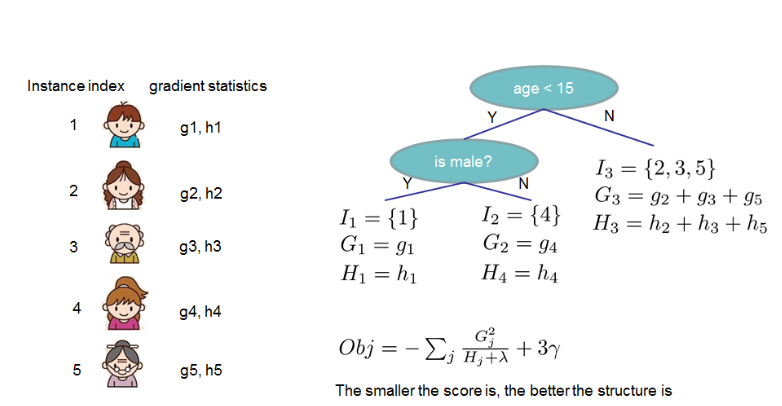
\includegraphics[scale=0.4]{images/estrutura_score_xgboost.png}
\end{figure}

CatBoost (para “impulsionamento categórico”) concentra-se em colunas categóricas usando técnicas de permutação, one\_hot\_max\_size (OHMS) e estatísticas baseadas em alvo. CatBoost resolve o crescimento exponencial da combinação de recursos usando o método greedy em cada nova divisão da árvore atual. Além disso a construção é feita por arvores simétricas e o algoritmo suporta colunas categóricas \cite{article:catboost,doc:catboost}.

O LightGBM é parecido com o XGBoost com algumas alterações: uma nova técnica para estimar o ganho de informação chamada \textit{gradient-based one-side sampling} (GOSS). Uma vez que uma das tarefas mais demoradas no processo de aprendizagem no aumento de gradiente é encontrar a divisão para as árvores, geralmente algum tipo de amostragem é feito nesta etapa para fins de eficiência \cite{article:lgbm,doc:LGBM}.

Temos abaixo um comparativo com maiores detalhes de cada algoritmo.
\subsection{Divisões de nó}
Antes de começar o aprendizado os algortimos precisam criar pares de divisões de recursos, por exemplo (idade,$<15$), (idade,$>20$), (quantidade, >1000). Esses pares de divisão de recurso são construídos com base em histograma e são usados durante o processo de aprendizado como possíveis divisões de nó. Esse método de pré-processamento é mais rápido do que o algoritmo \textit{greedy}, que enumera linearmente todas as divisões possíveis para recursos contínuos.

O \textbf{XGboost} não utiliza nenhuma técnica de amostragem ponderada, ele utiliza algoritmos puramente baseados em histogramas o que torna seu processo de divisão mais lento em comparação com GOSS e MVS.

O \textbf{Catboost} oferece uma nova técnica chamada \textit{Minimal Variance Sampling} (MVS), que é uma versão de amostragem ponderada do \textit{Stochastic Gradient Boosting}. Nesta técnica, a amostragem ponderada ocorre no nível da árvore e não no nível da divisão. As observações para cada árvore de reforço são amostradas de forma a maximizar a precisão da pontuação dividida.

O \textbf{LightGBM} oferece amostragem unilateral baseada em gradiente (GOSS) que seleciona a divisão usando todas as instâncias com grandes gradientes (ou seja, grande erro) e uma amostra aleatória de instâncias com pequenos gradientes. Para manter a mesma distribuição de dados ao calcular o ganho de informação, o GOSS introduz um multiplicador constante para as instâncias de dados com pequenos gradientes. Assim, o GOSS consegue um bom equilíbrio entre aumentar a velocidade, reduzindo o número de instâncias de dados, e manter a precisão das árvores de decisão aprendidas.

\subsection{Crescimento da Árvore}
O \textbf{XGboost} divide as árvores até o hiperparâmetro max\_depth especificado e logo em seguida começa a podar a árvore para trás e remove as divisões além das quais não há ganho positivo. Ele usa essa abordagem, pois às vezes uma divisão sem redução de perda pode ser seguida por uma divisão com redução de perda. O XGBoost também pode executar o crescimento da árvore folha a folha (como LightGBM).

\textbf{Catboost} cresce uma árvore equilibrada. Em cada nível dessa árvore, o par de divisão de recursos que traz a menor perda (de acordo com uma função de penalidade) é selecionado e é usado para todos os nós do nível. É possível alterar sua política usando o parâmetro grow\_policy.

O \textbf{LightGBM} usa crescimento de árvore folha a folha (melhor primeiro). Opta por cultivar a folha que minimiza a perda, permitindo um crescimento de uma árvore desequilibrada. Como não cresce em nível, mas em folha, o \textit{overfitting} pode acontecer quando os dados são pequenos. Nesses casos, é importante controlar a profundidade da árvore.

A figura \ref{fig:three graphs} mostra o comparativo do crescimento de árvore de cada algoritmo.

\begin{figure}[H]
     \centering
     \begin{subfigure}[b]{0.4\textwidth}
         \centering
         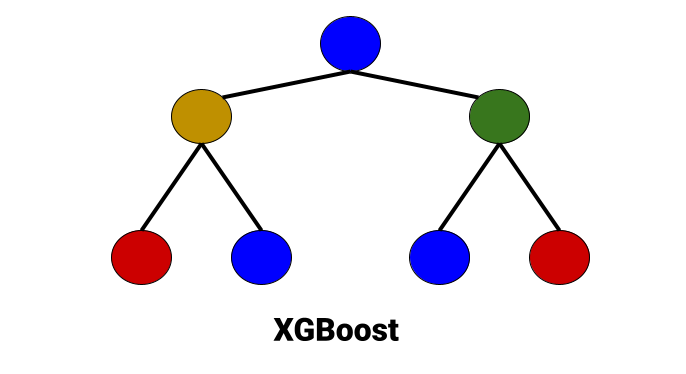
\includegraphics[width=\textwidth]{images/XGboost.png}
     \end{subfigure}
     \hfill
     \begin{subfigure}[b]{0.4\textwidth}
         \centering
         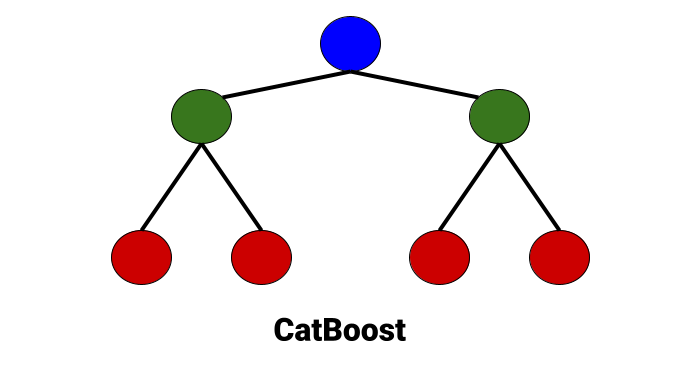
\includegraphics[width=\textwidth]{images/CatBoost.png}
     \end{subfigure}
     \hfill
     \begin{subfigure}[b]{0.4\textwidth}
         \centering
         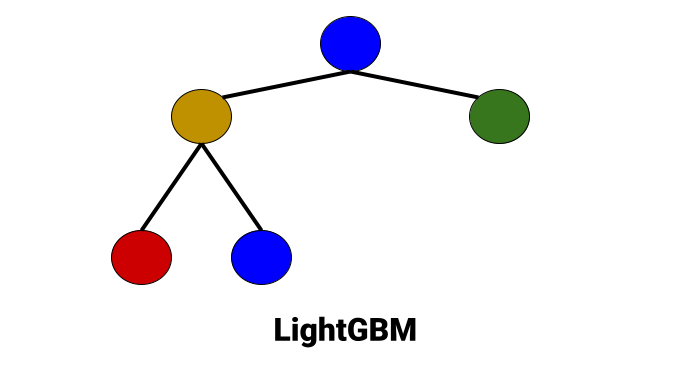
\includegraphics[width=\textwidth]{images/LGBM.png}
     \end{subfigure}
        \caption{Comparativo do crescimento da Árvore no XGBoost, CatBoost e LightGBM}
        \label{fig:three graphs}
\end{figure}


\subsection{Valores \textit{Missing}}
No \textbf{XGboost} e \textbf{LightGBM}, os valores \textit{missing} serão alocados para o lado que reduz a perda em cada divisão. Enquanto o \textbf{Catboost} tem dois modos para processar valores ausentes, “Min” e “Max”. Em “Min”, os valores ausentes são processados como o valor mínimo para um recurso (eles recebem um valor menor que todos os valores existentes). Dessa forma, é garantido que uma divisão que separa os valores ausentes de todos os outros valores seja considerada ao selecionar as divisões. “Max” funciona exatamente da mesma forma que “Min”, apenas com valores máximos.

\subsection{\textit{Feature Importance}}
O \textbf{XGboost} e o \textbf{LightGBM} têm dois métodos semelhantes: O primeiro é “Ganho”, que foi explicado na equação \ref{eq:gain}. É a melhoria na precisão (ou ganho total) trazida por um recurso para os ramos em que está. O segundo método tem um nome diferente em cada pacote: \textit{split} (LightGBM) e \textit{Frequency/Weight} (XGBoost). Este método calcula o número relativo de vezes que um determinado recurso ocorre em todas as divisões das árvores do modelo. Esse método pode ser influenciado por recursos categóricos com um grande número de categorias.

O \textbf{XGboost} possui mais um método, \textit{Coverage}, que é o número relativo de observações relacionadas a uma feição. Para cada recurso, contamos o número de observações usadas para decidir o nó folha.

\textbf{Catboost} tem dois métodos: O primeiro é \textit{PredictionValuesChange}. Para cada recurso, \textit{PredictionValuesChange} mostra quanto, em média, a previsão muda se o valor do recurso mudar. Uma característica teria uma importância maior quando uma mudança no valor da característica causa uma grande mudança no valor previsto. Este é o método de cálculo de importância de recurso padrão para métricas não classificadas. O segundo método é \textit{LossFunctionChange}. Esse tipo de importância de recurso pode ser usado para qualquer modelo, mas é particularmente útil para modelos de classificação. Para cada característica o valor representa a diferença entre o valor de perda do modelo com esta característica e sem ela. Como é computacionalmente caro retreinar o modelo sem um dos recursos, esse modelo é construído aproximadamente usando o modelo original com esse recurso removido de todas as árvores do conjunto. O cálculo dessa importância de recurso requer um conjunto de dados.

\subsection{Variáveis Categóricas}
O \textbf{XGboost} não possui um método embutido para recursos categóricos. A codificação (\textit{one-hot-encoding}, codificação de destino, etc.) deve ser realizada pelo usuário.

\textbf{Catboost} usa uma combinação de codificação one-hot e uma codificação média avançada. Para recursos com baixo número de categorias, ele usa \textit{one-hot-encoding}. O número máximo de categorias para \textit{one-hot-encoding} pode ser controlado pelo parâmetro one\_hot\_max\_size. Para as colunas categóricas restantes, CatBoost usa um método eficiente de codificação, que é semelhante à codificação média, mas com um mecanismo adicional destinado a reduzir o \textit{overfitting}.

\textbf{LightGBM} divide recursos categóricos particionando suas categorias em 2 subconjuntos. A ideia básica é classificar as categorias de acordo com o objetivo do treinamento em cada divisão, o valor final que vai ser treinado no modelo tem que ser um valor númerico.

A Tabela \ref{tabela:ex:dif:algo} resume essas principais diferenças entre os algoritmos.
\begin{table}[H]
\centering
\caption{Principais características do XGBoost, CatBoost e LightGBM}
\label{tabela:ex:dif:algo}
\begin{tabular}{|p{4cm}|p{3cm}|p{3cm}|p{3cm}|} 
 \hline
& \textbf{XGBoost} & \textbf{CatBoost} & \textbf{LightGBM} \\
  \hline
  \textbf{Desenvolvedor} & DMLC & Yandex & Microsft \\
  \hline
  \textbf{Ano de Release} & 2014 & 2017 & 2016 \\
  \hline
  \textbf{Simetria da Árvore} & Assimétrica Level-wise  & Simétrica & Assimétrica Leaf-wise \\
  \hline
  \textbf{Método de Splitting} & Algoritmos de histogramas & Greedy & GOSS \\
  \hline
  \textbf{Colunas Numéricas} & Suporta & Suporta & Suporta \\
  \hline
  \textbf{Colunas Categóricas} & Não Suporta (conveter utilizando one-hot-encoding) & Suporta & Não Suporta (converter para numérico ou ordinal) \\
  \hline
  \textbf{Colunas de Texto} & Não Suporta & Suporta & Não Suporta \\
  \hline
  \textbf{Valores missing} & Interpreta como NaN ou zero & Interpreta como NaN ou zero & Interpreta como NaN ou zero \\
  \hline
\end{tabular}
\end{table}

\section{Hiperparâmetros} \label{cap3:hiper}
Conforme vimos na seção anterior, uma das principais diferença entre o XGBoost e CatBoost para o LGBM é que o LGBM cultiva folhas de árvores, enquanto que os outros algoritmos utilizam uma abordagem de profundidade. Isso impacta em como cada valor de hiperparâmetro deve ser escolhido e quais valores devem ser otimizados e estudados. Cada algoritmo pode ter mais de 20 hiperparâmetros. Abaixo temos os hiperparâmetros mais comuns e alguns deles serão analisados na primeira parte desse estudo. Na segunda parte, ao utilizar o Optuna para tunar o modelo podemos inserir mais hiperparâmetros.
\begin{itemize}
    \item \textbf{learning\_rate:} Taxa de aprendizado $\eta$, é o parâmetro que discutimos em \ref{eq:gradiente}, ele é responsável por controlar a influencia de cada novo aprendiz, ou seja, ele basicamente determina o tamanho do passo de cada interação enquanto se move em direção a um mínimo da função de perda.
    \item \textbf{num\_leaves:}Este hiperparâmetro controla o número máximo de folhas a crescer em cada iteração, e é a principal forma de controlar a complexidade do modelo.
    \item \textbf{max\_depth:} Profundidade máxima de uma árvore. Aumentar esse valor tornará o modelo mais complexo e com maior probabilidade de \textit{overfit}.
    \item \textbf{n\_estimators:} O número de estimadores ou iterações de aumento no processo de aumento de gradiente. Isto é o parâmetro $M$ na Equação \ref{eq:interacoes} e controla quantas árvores são cultivadas no treinamento do modelo. Normalmente, quanto maior o número de iterações, melhor o modelo ficará, até que comece \textit{overfitting} nos dados de treinamento.
    \item \textbf{early\_stopping\_rounds:} É um parâmetro utilizado para reduzir o \textit{overfitting} ele recebe um valor inteiro que informa ao algoritmo quando parar se não houver mais melhorias na métrica de avaliação. Pode evitar o \textit{overfitting} e melhorar o desempenho do seu modelo. Não necessariamente é um parâmetro que queremos 'tunar', mas vamos utilizar ele para reduzir o \textit{overfitting}.
    \item \textbf{reg\_lambda:} Termo de regularização $L2$ nos pesos.
\end{itemize}

\section{Optuna}
Uma das tarefas mais importantes na construção de modelos de aprendizado de máquina é a otimização de hiperparâmetros. Uma otimização correta dos hiperparâmetros se reflete diretamente no desempenho do modelo e nos últimos anos essa frente de otimização dos hiperparâmetros tem tido grande avanço na pesquisa e diversas soluções existem atualmente. Podemos citar Spearmint, Vizer, AutoSklearn, HyperOpt, dentre outras. Entretanto cada ferramente propõe uma própria abordagem de usabilidade podendo se tornar mais ou menos flexível dependo do caso ou complexidade do modelo. Ou seja, a escalabilidade dessas aplicações pode ser dificultada. Com isso, surgiu o Optuna um framework Open Source para otimização de hiperparâmetros, cujo objetivo é unificar os paradigmas de otimização sob uma filosofia apoiada em três pilares: \textit{API design-by-run}, implementação eficiente, facilidade de configuração e versatilidade de arquitetura \cite{optuna}\cite{doc:optuna}.

Na Tabela \ref{tabela:ex:dif:optuna} temos uma comparação de outros algoritmos de otimização de hiperparâmetros e o Optuna \cite{optuna}.
\begin{table}[h]
\centering
\caption{Comparativo de outros algorítimos de otimização de hiperparâmetros \cite{optuna}.}
\label{tabela:ex:dif:optuna}
\begin{tabular}{|c|c|c|c|c|c|c|} 
 \hline
\textbf{Framework} & \textbf{API} & \textbf{Pruning} & \textbf{Lightweight} & \textbf{Distributed} & \textbf{Dashboard} & \textbf{OSS}\\
  \hline
  SMAC & define and run     & \xmark & \cmark & \xmark & \xmark &\cmark\\
  \hline
  GPyOpt & define and run   & \xmark & \cmark & \xmark & \xmark &\cmark\\
  \hline
  Spearmint & define and run & \xmark & \cmark & \cmark & \xmark &\cmark\\
  \hline
  Hyperopt & define and run & \xmark & \cmark & \cmark & \xmark &\cmark\\
  \hline
  Autotune & define and run & \cmark & \xmark & \cmark & \cmark &\xmark\\
  \hline
  Vizier & define and run & \cmark & \xmark & \cmark & \cmark &\xmark\\
  \hline
  Katib & define and run & \cmark & \xmark & \cmark & \cmark &\cmark\\
  \hline
  Tune & define and run & \cmark & \xmark & \cmark & \cmark &\cmark\\
  \hline
  Optuna & define by run & \cmark & \cmark & \cmark & \cmark &\cmark\\
  \hline
\end{tabular}
\end{table}

Por padrão o Optuna utiliza Tree-Structured Parzen Estimator, um algorítimo de otimização Bayesiana, conforme foi abordado no capitulo \ref{chapter:fundamentos-aprendizado}, mas podem ser utilizados outros algoritmos de otimização. Para mais informações sobre esse tipo de otimização e os outros algoritmos consulte \cite{doc:optuna,hyper:op:theory,grid:book,neural:op,op:TPE}.

Antes de começar a implementar a otimização com Optuna, é necessário definir uma função objetivo. A função objetivo conterá toda a lógica de um processo regular de definição, treinamento e teste de modelo. Após a avaliação do modelo, ele deve retornar a métrica de avaliação que também é escolhida pelo usuário.
A classe Trial será usada para armazenar informações de uma combinação específica de hiperparâmetros usados posteriormente pelo modelo de aprendizado de máquina.
Um objeto de estudo pode então ser chamado para otimizar a função objetivo para encontrar a melhor combinação de hiperparâmetros. Em seguida, ele executará testes iterativamente até um teste ou tempo máximo definido pelo usuário. O ensaio com os melhores hiperparâmetros será armazenado em study.best\_trial.

\begin{codigo}[caption={Definição de uma função objetivo e o processo de otimização no Optuna}, label={codigo:ex:optuna}, language=Python, breaklines=true]
import optuna

def objective(trial):
    x = trial.suggest_float('x', -10, 10)
    return (x - 2) ** 2

study = optuna.create_study()
study.optimize(objective, n_trials=100)
trial = study.best_trial
print("Best Trial: ", trial.value)
\end{codigo}

Uma das principais vantagens do Optuna é sua estrutura avançada de visualizações para a interpretação de todo o processo de otimização, podemos utilizar a biblioteca para entender a relação entre os hiperparâmetros.

Além disso, o Optuna é projetado para facilidade de implementação, flexibilidade e escalabilidade. A otimização de experimentos em larga escala, por exemplo, pode ser realizada de maneira paralela e distribuída. Optuna é framework agnóstico, ou seja, pode ser facilmente integrado com qualquer um dos frameworks de aprendizado de máquina e aprendizado profundo, como: PyTorch, Tensorflow, Keras, Scikit-Learn, XGBoost, LGBM e etc.

\begin{figure}[H]
 \caption{Arquitetura do Optuna}
 \label{fig:arq:optuna}
 \centering
 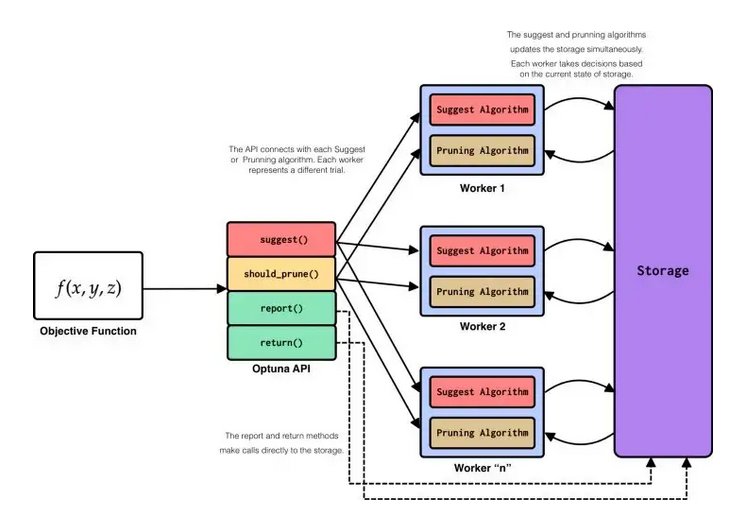
\includegraphics[scale=0.3]{images/arquitetura_optuna.png}
\end{figure}

\section{\textit{SHAP e Shapley Values}}
Entender a importância das variáveis de um modelo predito é um conceito extremamente necessário e importante. As variáveis podem explicar a dinâmica do problema no mundo real, que em muitos casos são desconhecidas, aprimorando o conhecimento do 
 do problema para o cientista de dados ou pesquisadores envolvidos na construção do modelo. Também podem ser usadas para auditar modelos complexos e entender se o modelo não está discriminando algo errado \cite{article:tec:interpr}.

 Essa tarefa é extremamente complexa, pois como vimos os modelos que vamos utilizar neste estudo, GBMs, fazem diversas operações no conjunto de dados, inclusive operações não-lineares. Isso torna a quantificação da importância de cada variável extremamente complexa.

\textit{SHAP (SHapley Additive exPlanations)} é uma abordagem que vem da teoria de jogos para explicar a saída de qualquer modelo de aprendizado de máquina. Ele conecta a saída do modelo com as explicações locais usando os valores de Shapley. A principal ideia do SHAP é criar um modelo mais simples, para que se possa explicar as como as variáveis locais impactam no modelo final \cite{shap:article,shap:article2,shap:doc}.

\begin{figure}[H]
 \caption{Exemplo do SHAP mostrando a importância de cada variável de entrada na saída do modelo \cite{shap:doc}.}
 \label{fig:ex:shap}
 \centering
 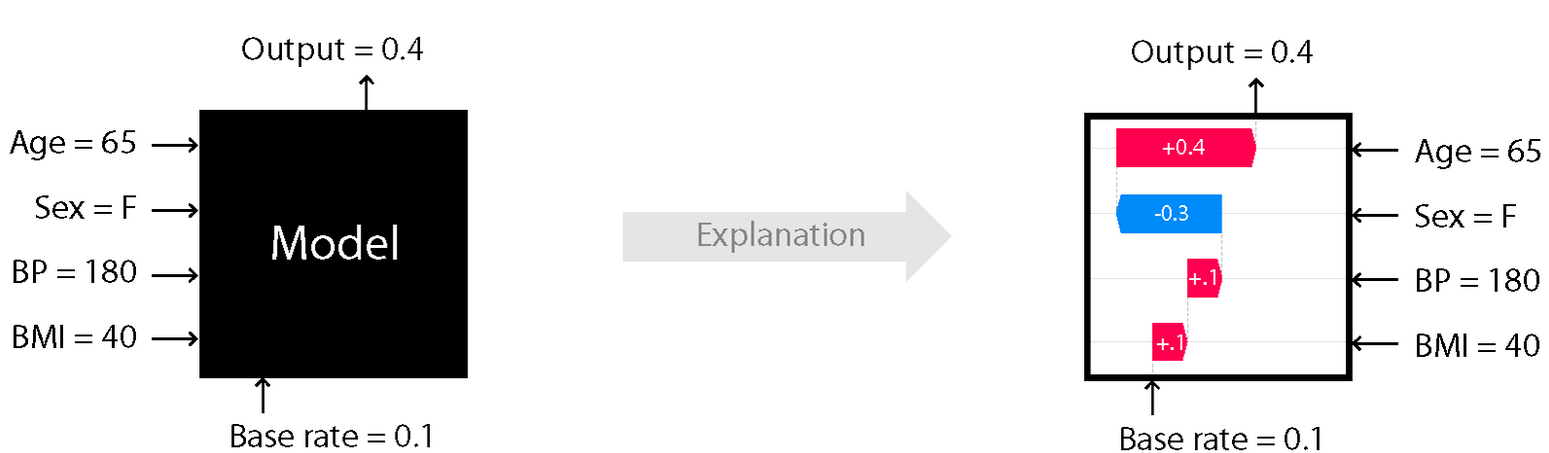
\includegraphics[scale=0.2]{images/exemplo_shap_black.png}
\end{figure}

\begin{figure}[H]
 \caption{Esquemático de como usar o SHAP para interpretar as predições do modelo \cite{iee:artigo:shap}}.
 \label{fig:ex:shap2}
 \centering
 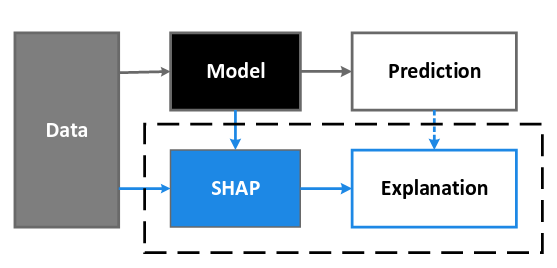
\includegraphics[scale=0.4]{images/over_shap.png}
\end{figure}

Estes métodos têm um modelo de explicação que é uma função linear de variáveis binárias:

\begin{equation}
    g(z') = \phi_{0} + \sum_{i=1}^{M} \phi_{i}z'_{i}
\end{equation}

Em que $z'\in \{0,1\}^M$, $M$ é o número de características de entrada simplificada e $\phi_i\in\mathbb{R}$. Os métodos atribuem um efeito $\phi_i\in\mathbb{R}$ a cada variável e a soma de todos os efeitos se aproxima do modelo original que queremos explicar. Uma das maiores contribuições do SHAP é propor a sua própria lógica de computar estes valores que garantem que eles tenham outras propriedades interessantes além do seu somatório aproximar a resposta do modelo original. E toda esta lógica surge dos \textit{Shapley Values}.


Os \textit{Shapley Values} foram introduzidos por Lloyd Shapley, no contexto da teoria dos jogos. Para um jogo cooperativo qualquer, os \textit{Shapley Values} distribuem uma quantidade total de contribuição para cada jogador da equipe de forma justa, ou seja tenta quantificar a contribuição individual para o ganho total \cite{shapley}. Em aprendizado de máquina, os valores de Shapley são a contribuição média de um valor de feature para a previsão total \cite{iee:artigo:shap}.

\begin{equation}
    \phi_i(f,x') = \sum_{z'\subseteq x'} \frac{|z'|!(M-|z'|-1)!}{M!}[f_x(z')-f_x(z'\setminus i)]
\end{equation}

\begin{figure}[H]
 \caption{SHAP valores atribuem a cada feição a mudança na previsão do modelo esperado ao condicionar esse recurso. Eles explicam como chegar do valor base $E[f (z)]$ que seria previsto se não conhecêssemos nenhum recurso para a saída atual $f(x)$. Este diagrama mostra um único pedido. Quando o modelo é não linear ou as características de entrada são não independentes, no entanto, a ordem em que os recursos são adicionados à expectativa importa, e os valores SHAP surgem da média dos valores $\phi_i$ em todas as ordenações possíveis. \cite{shap:article}}.
 \label{fig:ex:shap2}
 \centering
 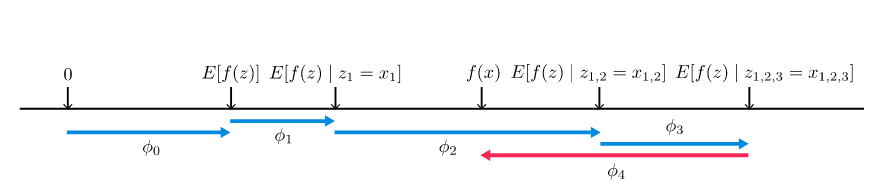
\includegraphics[scale=0.4]{images/shap_value_artigo.png}
\end{figure}

\begin{figure}[H]
 \caption{Gráfico do SHAP para o dataset Boston Housing.}.
 \label{fig:ex:shap_housing}
 \centering
 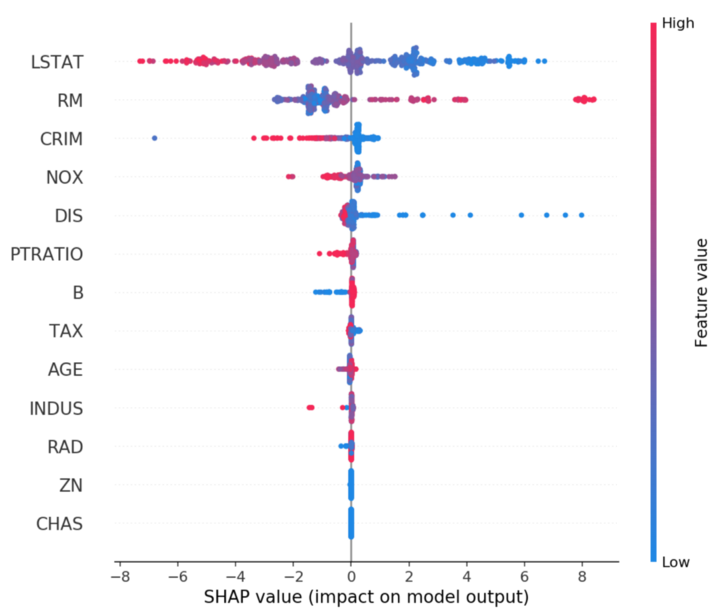
\includegraphics[scale=0.4]{images/shap_example_house.png}
\end{figure}

